\documentclass[10pt]{article}
\usepackage[a4paper,margin=0.82in]{geometry}
\usepackage{amsmath,amssymb}
\usepackage{graphicx}
\usepackage{booktabs,tabularx,array,longtable}
\usepackage{caption}
\usepackage{subcaption}
\usepackage{float}
\usepackage{enumitem}
\usepackage{xcolor}
\usepackage{microtype}
\usepackage{hyperref}
\hypersetup{colorlinks=true,linkcolor=blue,citecolor=blue,urlcolor=blue}
\newcommand{\mmals}{\textsc{MMALS}}
\newcommand{\rc}{\textsc{RC2O}}
\newcommand{\core}{\textsc{CORe50}}
\newcommand{\scx}{\textsc{SplitCIFAR10}}
\newcommand{\scxx}{\textsc{SplitCIFAR100}}
\title{\textbf{MMALS v1.1: From Functional-Memory Diagnostics to External Continual-Learning Evidence}\\
\large RC2O-v2.2c SplitCIFAR10 Qualification, SplitCIFAR100 and CORe50 Diagnostics, and the v2.3 Context-Retention Rescue}
\author{Guillaume Harbonnier\\MMALS Research Program}
\date{Status update: June 12, 2026}
\begin{document}
\maketitle

\begin{abstract}
Mycelium-Inspired Mutualistic Adaptive Learning Systems (\mmals{}) is a continual-learning research program organized around inferred context, functional routing, specialist hosts, replay and prototype memory, and explicit audit traces. This status article consolidates the path from MNIST-family functional-memory diagnostics to the latest external visual experiments. On \scx{}, the five-seed \rc{}-v2.2c bridge reaches $0.91395\pm0.00639$ final average accuracy, versus $0.73860\pm0.01559$ for validation-selected replay, with paired gain $+0.17535$ and 95\% confidence interval $[0.16093,0.18977]$. On \scxx{}, selected \rc{} reaches $0.53556\pm0.06207$ versus $0.33254\pm0.00742$ for replay, but the representation/control ladder fails qualification. On a custom five-seed \core{} object-level $10\times5$ stream, selected \rc{} reaches $0.31490\pm0.0345$ versus approximately $0.2796$ for replay, while severe early-task and old-context collapse prevents qualification. A two-seed v2.3 rescue ablation raises average accuracy from $0.2734$ to $0.3171$, minimum-task accuracy from $0.0050$ to $0.0513$, reduces mean zero-recall classes from $9.0$ to $0.5$, and breaks a one-host collapse; however, oldest-context top-1 remains zero, so the promotion gate fails. The evidence supports a robust external bridge on \scx{}, positive but bounded diagnostics on \scxx{} and \core{}, and a localized redesign of context-memory fusion. It does not establish end-to-end raw-pixel continual representation learning, state-of-the-art performance, positive backward transfer, or universal dataset generality.
\end{abstract}

\section{Research question and contribution}
The original \mmals{} question was not simply whether a modular neural network can achieve high classification accuracy. It was whether a learning medium can preserve useful transformations, infer latent context, route signals through reusable specialist hosts, and expose enough evidence to explain why a policy was selected. The research program therefore treats continual learning as a coupled problem of stability, plasticity, context inference, functional specialization, and governance.

The present contribution is a full status consolidation. It connects four evidence strata:
\begin{enumerate}[leftmargin=*]
\item MNIST-family mechanism and geometry diagnostics;
\item a robust external bridge on \scx{};
\item harder but representation-limited evidence on \scxx{};
\item a failure-driven \core{} diagnosis followed by a targeted v2.3 rescue ablation.
\end{enumerate}

The article deliberately separates a result from its maturity. A positive paired gain does not automatically imply robust retention, functional specialization, or benchmark qualification.

\begin{figure}[H]
\centering
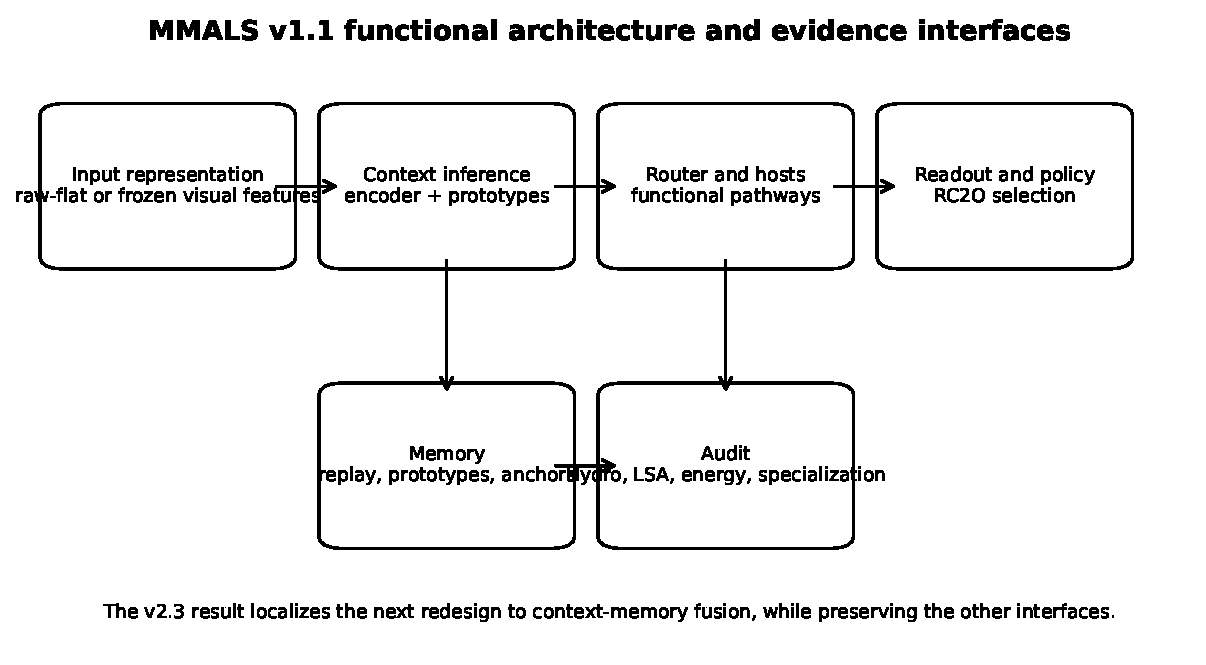
\includegraphics[width=0.96\linewidth]{figures/mmals_architecture_evolution.pdf}
\caption{The current \mmals{} architecture separates input representation, context inference, functional routing, memory, audit, and deployment policy. The newest evidence localizes the next redesign to the context-memory interface rather than requiring replacement of the full backbone.}
\end{figure}

\section{Architecture and learning object}
Let $e=\phi(x)$ be an input representation. For MNIST-family studies, $\phi$ can be the historical flattened input path. For external visual studies, $\phi$ is a frozen supervised feature extractor. Each host $H_k$ produces a transformed latent signal
\begin{equation}
 z_k = H_k(e), \qquad k=1,\ldots,K.
\end{equation}
A context posterior $q(c\mid e,m)$ and route vector $r(e,m,c)$ combine host outputs into a mediated latent state
\begin{equation}
 z_f = \sum_{k=1}^{K} r_k(e,m,c)\,T_k(z_k), \qquad \sum_k r_k=1,
\end{equation}
followed by a global readout $p(y\mid z_f)$. The memory object is not route topology alone. Earlier route-function disentanglement experiments showed that two systems may share almost identical routes while computing different latent functions. Accordingly, \mmals{} audits route drift, mediated latent drift, output drift, prototype geometry, learning-signal allocation, and host ablation.

The \rc{} controller is a validation-memory policy selector. It classifies the evidence regime and selects, locks, releases, falls back, or abstains among candidate policies. Final-test information is not used to trigger repair or choose the candidate.

\begin{figure}[H]
\centering
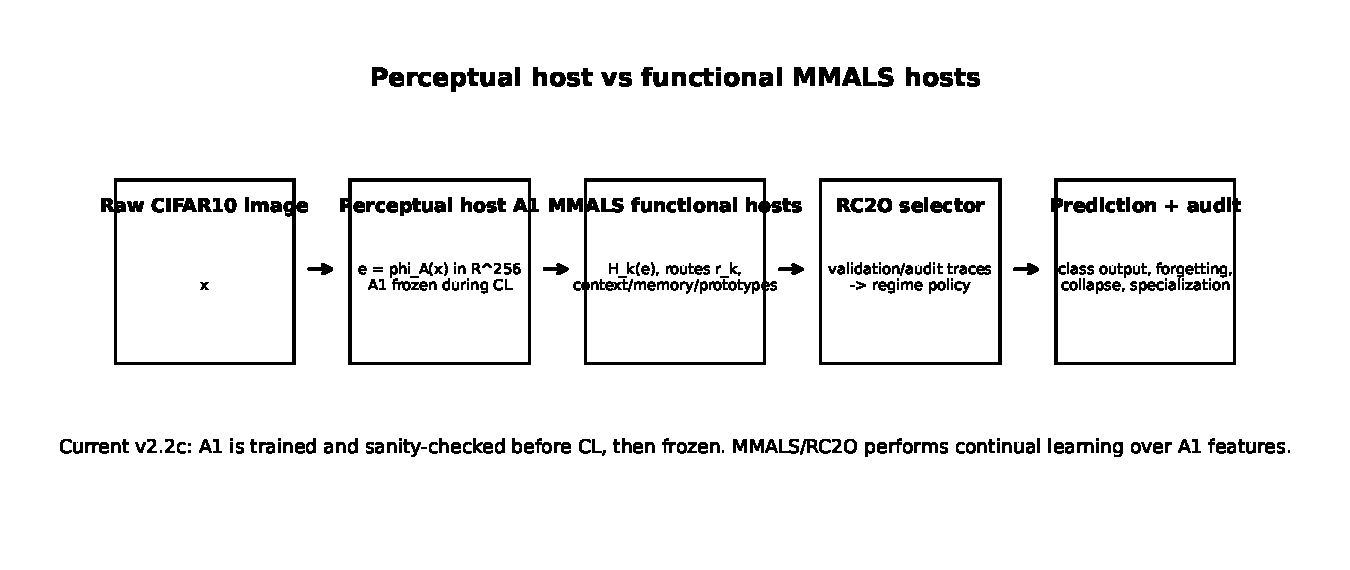
\includegraphics[width=0.93\linewidth]{figures/perceptual_host_pipeline.pdf}
\caption{External visual bridge used in v2.2c: a supervised perceptual host is frozen before the sequential continual-learning experiment; the downstream \mmals{} functional hosts, memory and \rc{} policy selector operate on the frozen features.}
\end{figure}

\section{Evidence discipline}
The program follows a progression of falsifiable gates rather than one aggregate score:
\begin{itemize}[leftmargin=*]
\item \textbf{Representation sanity:} determine whether failures originate upstream of continual learning.
\item \textbf{Baseline hardening:} select replay, EWC, LwF, PNN and MoE configurations using validation memory rather than arbitrary defaults.
\item \textbf{Retention evidence:} report average accuracy, minimum-task accuracy, forgetting, oldest-task performance, minimum-class recall and zero-recall classes.
\item \textbf{Context evidence:} report inferred-context accuracy, entropy, confusion, prototype separation and oracle-context gaps.
\item \textbf{Specialization evidence:} report effective hosts, route dominance, host ablation and host probes.
\item \textbf{Audit evidence:} retain Hydro, learning-signal alignment and energy probes as diagnostics unless explicitly activated for selection.
\end{itemize}

\begin{figure}[H]
\centering
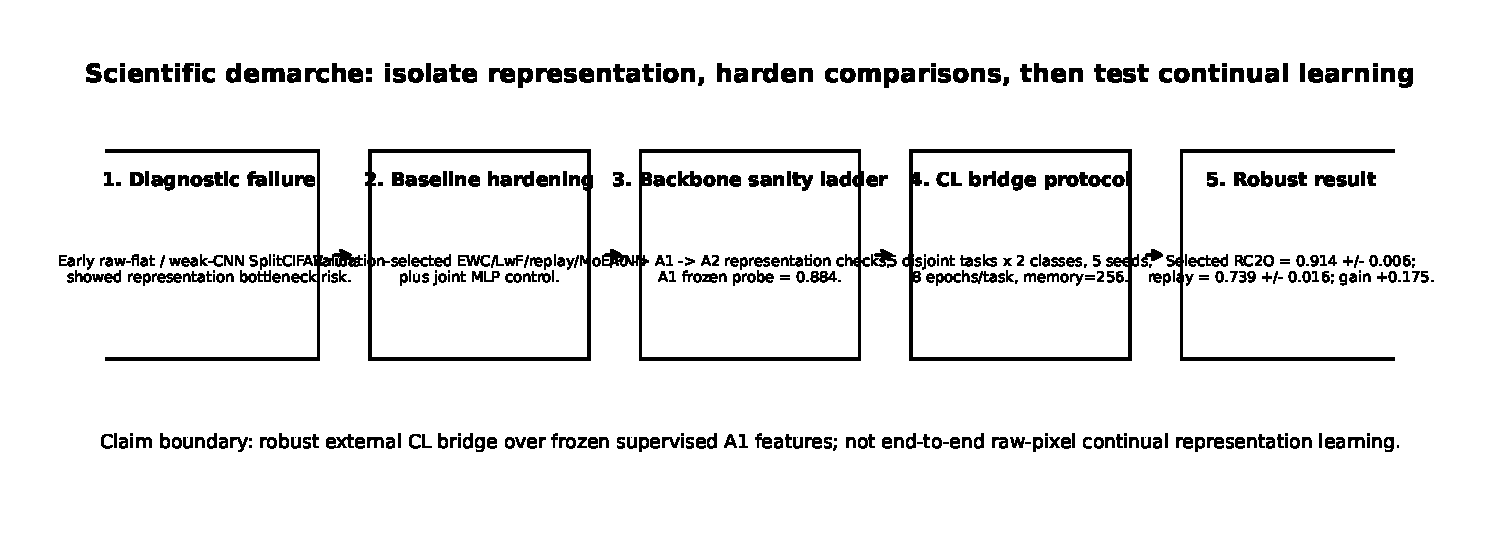
\includegraphics[width=0.98\linewidth]{figures/scientific_demarche_graph.pdf}
\caption{Scientific demarche used to move from representation debugging to bounded external continual-learning claims.}
\end{figure}

\section{MNIST-family foundations}
The MNIST-family branch established mechanisms before the external bridge. In v0.9, full functional memory reached approximately $0.9908$ final average accuracy with average forgetting near $5.25\times10^{-4}$. The main lesson was diagnostic: route preservation alone could leave large latent-function drift, whereas latent-preserving variants tracked retention more faithfully. In v0.12, the geometry/co-evolution branch reached approximately $0.9889$ final average accuracy and $0.0010$ average forgetting, but the additional geometry regularizer did not clearly outperform the full functional-memory reference. This was retained as a microscope rather than promoted as a performance claim.

The later v1.1 selector line moved from explicit task identity toward inferred context. Its qualitative regression targets remain important:
\begin{itemize}[leftmargin=*]
\item \textbf{MNIST:} clean context should permit a simple proto/global policy.
\item \textbf{FashionMNIST:} ambiguous overlap should preserve the guarded context-gap family.
\item \textbf{PermutedMNIST:} clean domain-shift evidence may release a true global guard.
\item \textbf{RotatedMNIST:} weak-boundary evidence may justify a generic latent calibration candidate.
\end{itemize}
These behaviors show why a future universal context-memory module must support soft ambiguity and backward-compatible legacy operation rather than forcing hard context separation everywhere.

\section{Consolidated evidence status}
\begin{table}[H]
\centering
\caption{Evidence strata and numerical status. Values across datasets are not direct difficulty-normalized rankings.}
\begin{tabularx}{\linewidth}{@{}l l r r r X@{}}
\toprule
Dataset / branch & Protocol & Selected & Replay & Oracle & Status \\
\midrule
MNIST-family v0.9 & 5-task functional-memory diagnostic & 0.9908 & -- & -- & Route-only memory was insufficient; functional latent preservation was supported diagnostically. \\
MNIST-family v0.12 & geometry / co-evolution diagnostic & 0.9889 & -- & -- & Very low forgetting, but no clear accuracy advantage of the geometry regularizer. \\
SplitCIFAR10 v2.2c & 5 tasks $\times$ 2 classes, 5 seeds & 0.9140 & 0.7386 & 0.9235 & Robust external-bridge qualification over frozen visual features. \\
SplitCIFAR100 v2.2c & 10 tasks $\times$ 10 classes, 5 seeds & 0.5356 & 0.3325 & 0.6551 & Positive robust diagnostic; representation/control gate not passed. \\
CORe50 v2.2c & custom 10 tasks $\times$ 5 objects, 5 seeds & 0.3149 & 0.2796 & 0.3631 & Positive diagnostic; severe old-task and old-context collapse. \\
CORe50 v2.3 & seeds 0 and 4, three rescue variants & 0.3171 & 0.2734 ref. & -- & Partial rescue: class and host collapse improved, oldest-context rescue failed. \\
\bottomrule
\end{tabularx}

\end{table}

\begin{figure}[H]
\centering
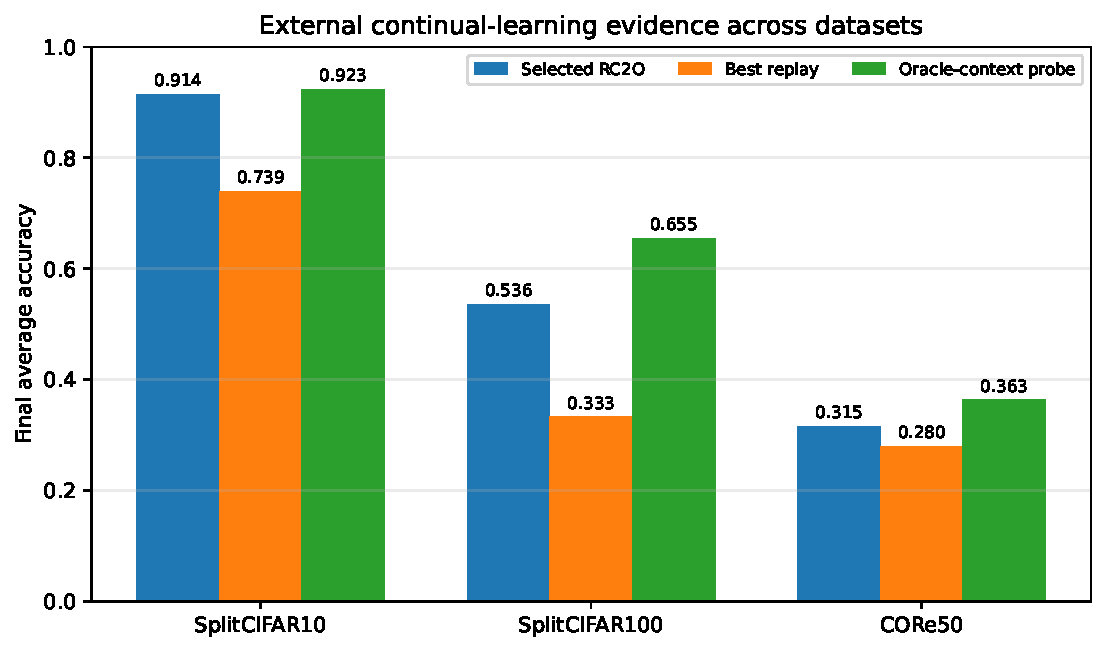
\includegraphics[width=0.88\linewidth]{figures/external_cross_dataset_comparison.pdf}
\caption{Selected \rc{}, replay and oracle-context probe on the three external visual studies. Dataset difficulty and protocol differ; the figure is a status comparison, not a normalized leaderboard.}
\end{figure}

\begin{figure}[H]
\centering
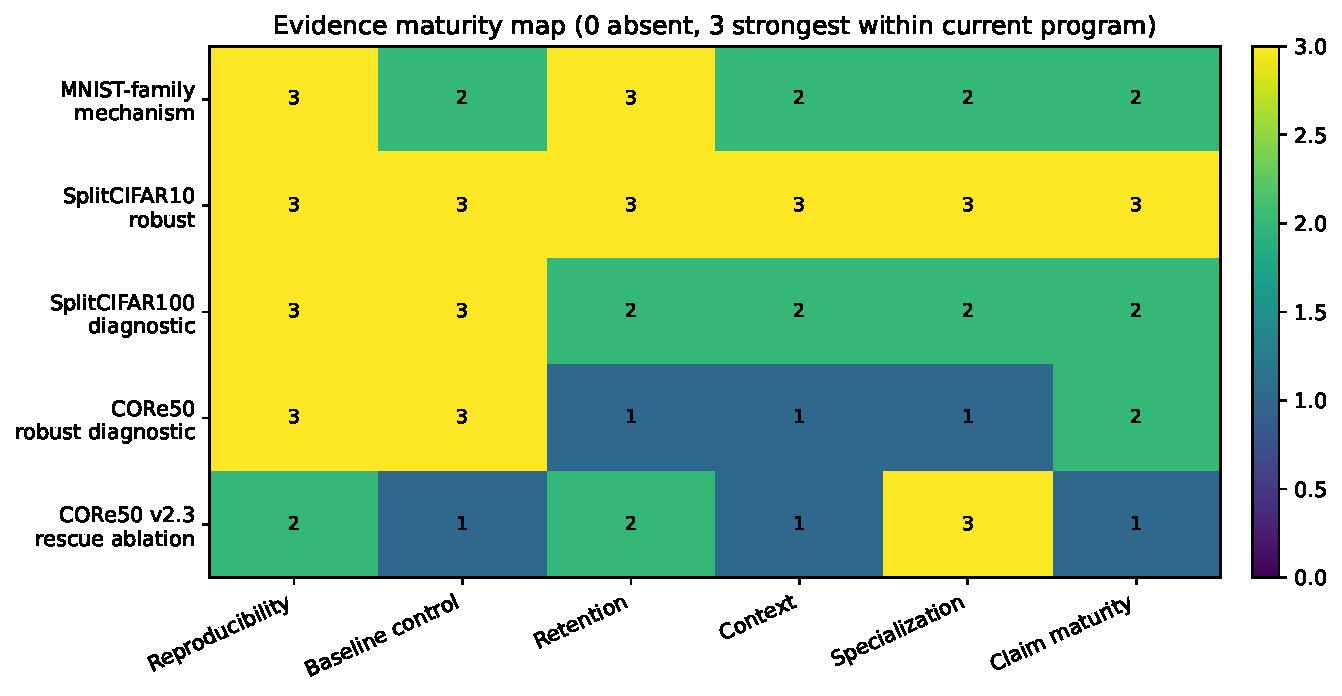
\includegraphics[width=0.92\linewidth]{figures/evidence_maturity_map.pdf}
\caption{Evidence maturity map. The scoring is an internal program summary, not a standardized benchmark metric.}
\end{figure}

\section{SplitCIFAR10: robust external bridge}
The \scx{} protocol uses five disjoint class-incremental tasks
\begin{equation}
(0,1)\rightarrow(2,3)\rightarrow(4,5)\rightarrow(6,7)\rightarrow(8,9).
\end{equation}
A supervised A1 visual backbone maps images to a frozen 256-dimensional representation. The downstream experiment spans five seeds, eight epochs per task and validation-selected baseline sweeps.

Selected \rc{} reaches $0.91395\pm0.00639$, compared with $0.73860\pm0.01559$ for the best replay baseline and $0.92345$ for the oracle-context probe. The paired gain over replay is positive in every seed and averages $+0.17535$ with 95\% confidence interval $[0.16093,0.18977]$. Minimum-task accuracy is $0.8535$, average forgetting is $0.02425$, minimum-class recall is $0.8410$, and no class has zero recall.

\begin{figure}[H]
\centering
\begin{subfigure}{0.48\linewidth}
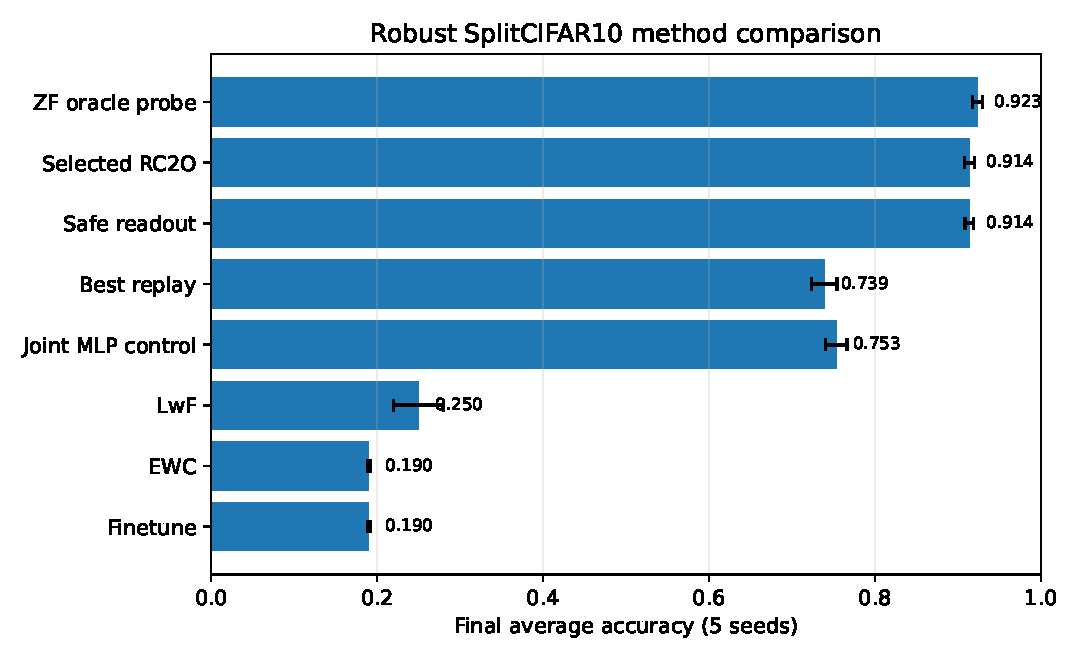
\includegraphics[width=\linewidth]{figures/splitcifar10_method_comparison.pdf}
\caption{Method comparison.}
\end{subfigure}\hfill
\begin{subfigure}{0.48\linewidth}
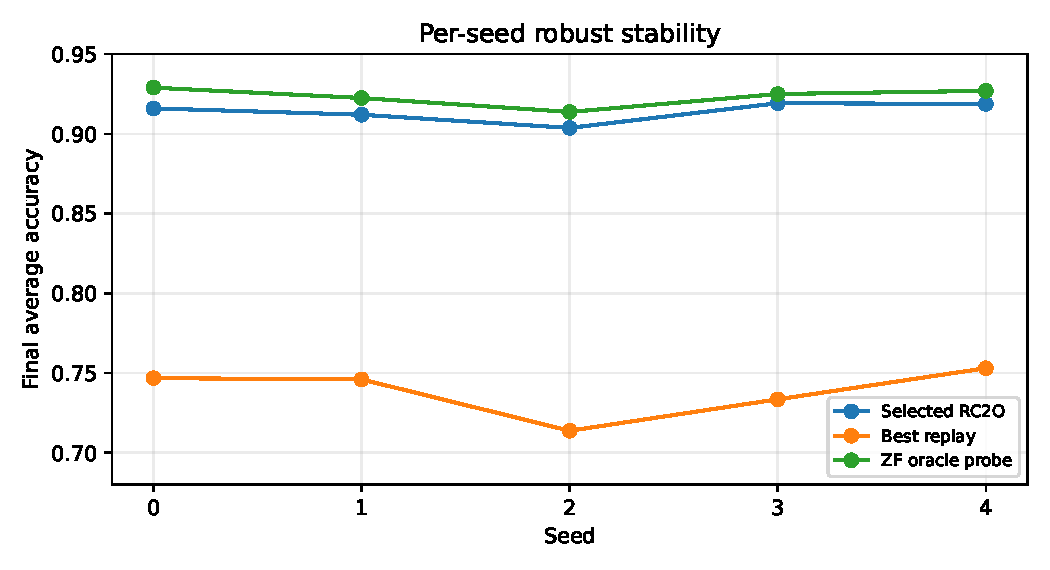
\includegraphics[width=\linewidth]{figures/splitcifar10_per_seed.pdf}
\caption{Per-seed stability.}
\end{subfigure}
\caption{\scx{} robust external-bridge result.}
\end{figure}

This is the strongest current non-MNIST result. The claim remains bounded: the visual representation is trained before the CL sequence and frozen. The experiment qualifies the downstream memory, routing, readout and selector bridge, not end-to-end continual feature acquisition.

\section{SplitCIFAR100: positive but representation-limited diagnostic}
The \scxx{} run uses ten tasks of ten classes. Selected \rc{} reaches $0.53556\pm0.06207$, compared with $0.33254\pm0.00742$ for replay. The paired gain is $+0.20302$ with 95\% confidence interval $[0.13431,0.27173]$. The safe readout reaches $0.53770$, while the oracle-context probe reaches $0.65506$.

\begin{figure}[H]
\centering
\begin{subfigure}{0.48\linewidth}
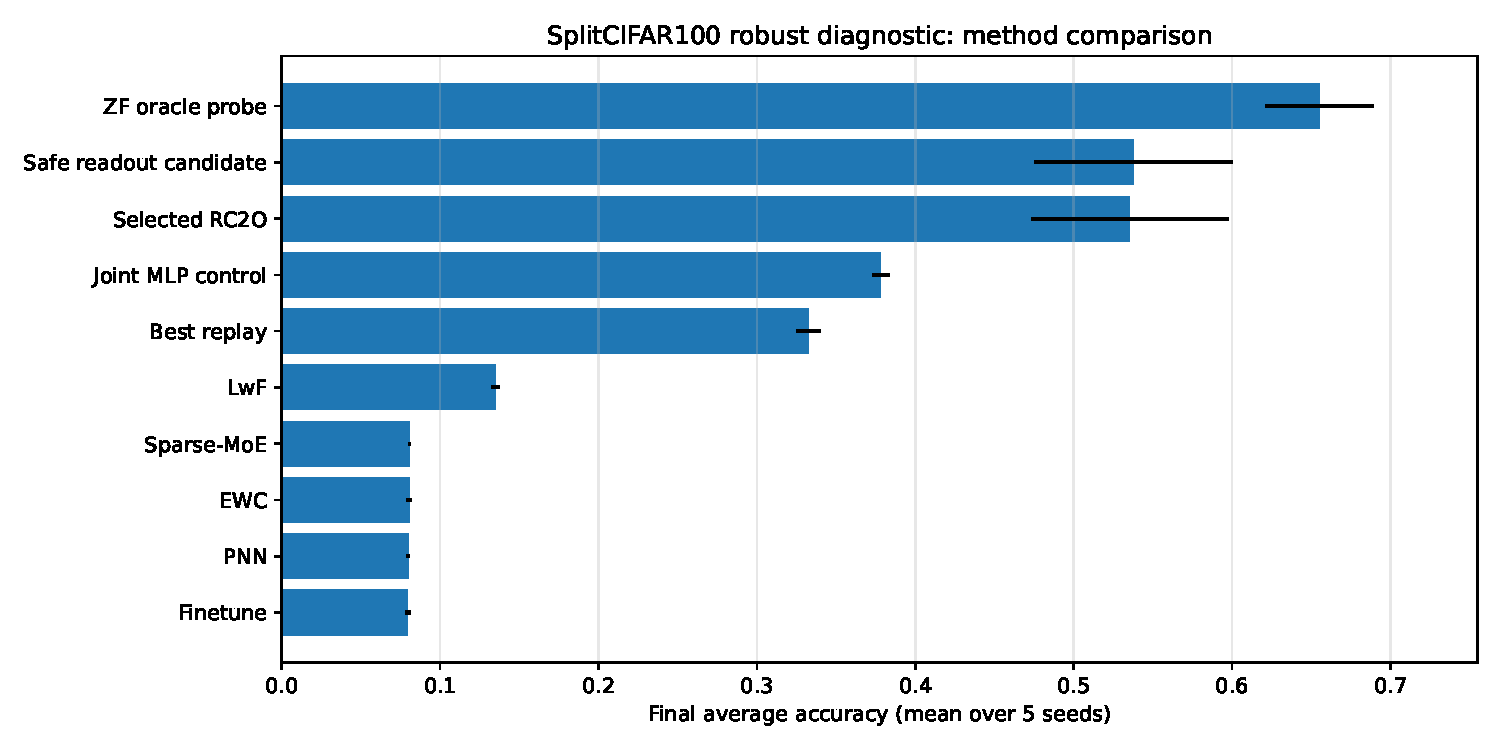
\includegraphics[width=\linewidth]{figures/splitcifar100_method_comparison.pdf}
\caption{Robust diagnostic comparison.}
\end{subfigure}\hfill
\begin{subfigure}{0.48\linewidth}
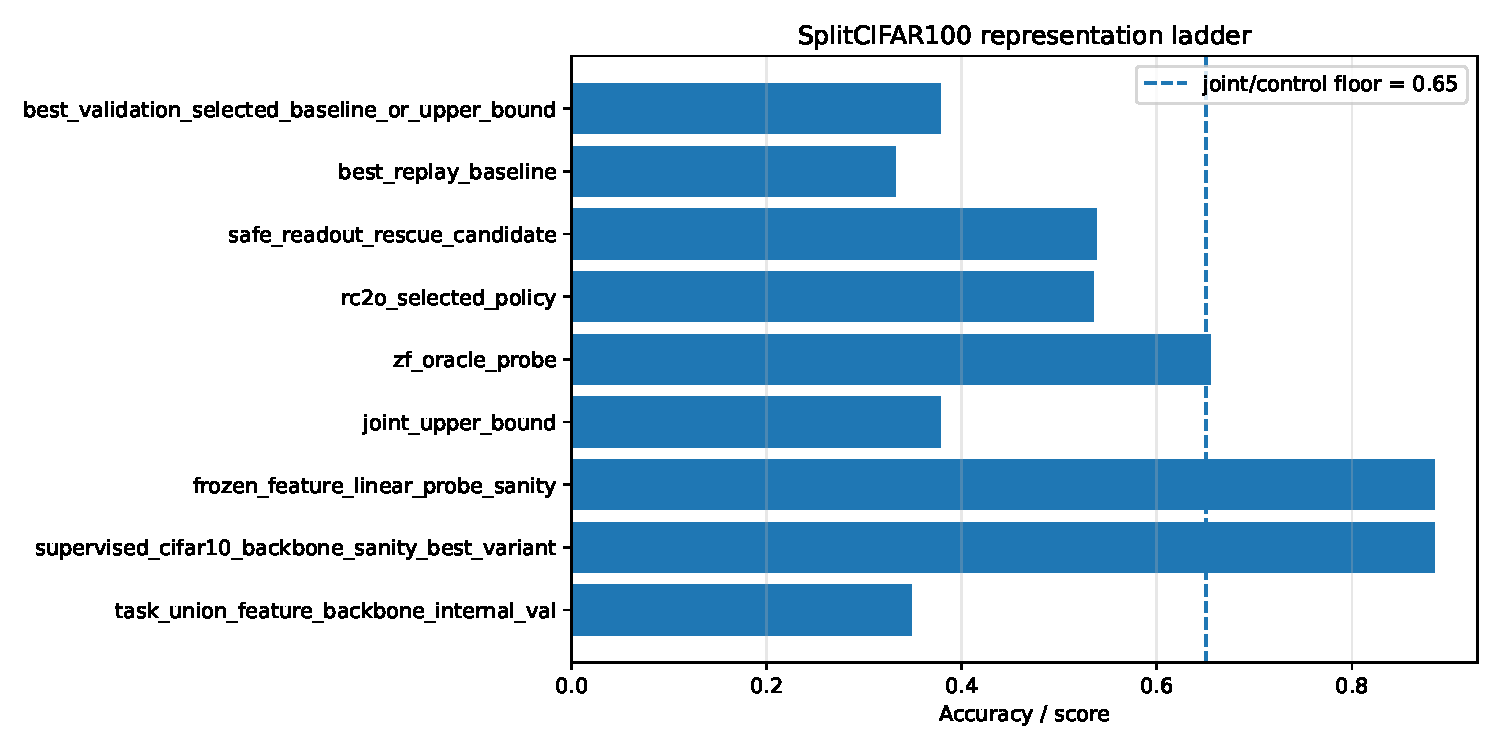
\includegraphics[width=\linewidth]{figures/splitcifar100_representation_ladder.pdf}
\caption{Representation/control ladder.}
\end{subfigure}
\caption{\scxx{} result and qualification bottleneck.}
\end{figure}

The joint MLP control reaches only $0.37824$, below the configured control floor. Therefore, the positive gain over replay is informative but cannot be separated cleanly from representation and readout limitations. The correct status is \emph{positive robust diagnostic}, not qualification.

\section{CORe50: transfer, failure and diagnosis}
The \core{} study uses a custom object-level stream of ten tasks with five object classes per task. The feature backbone is trained on train-only tensors, frozen, and followed by the same downstream \mmals{}/\rc{} pipeline. Across five seeds, selected \rc{} reaches $0.31490\pm0.0345$ and replay approximately $0.2796$. The paired gain is $+0.03529$ with 95\% confidence interval $[0.00292,0.06766]$, positive in every seed.

\begin{figure}[H]
\centering
\begin{subfigure}{0.48\linewidth}
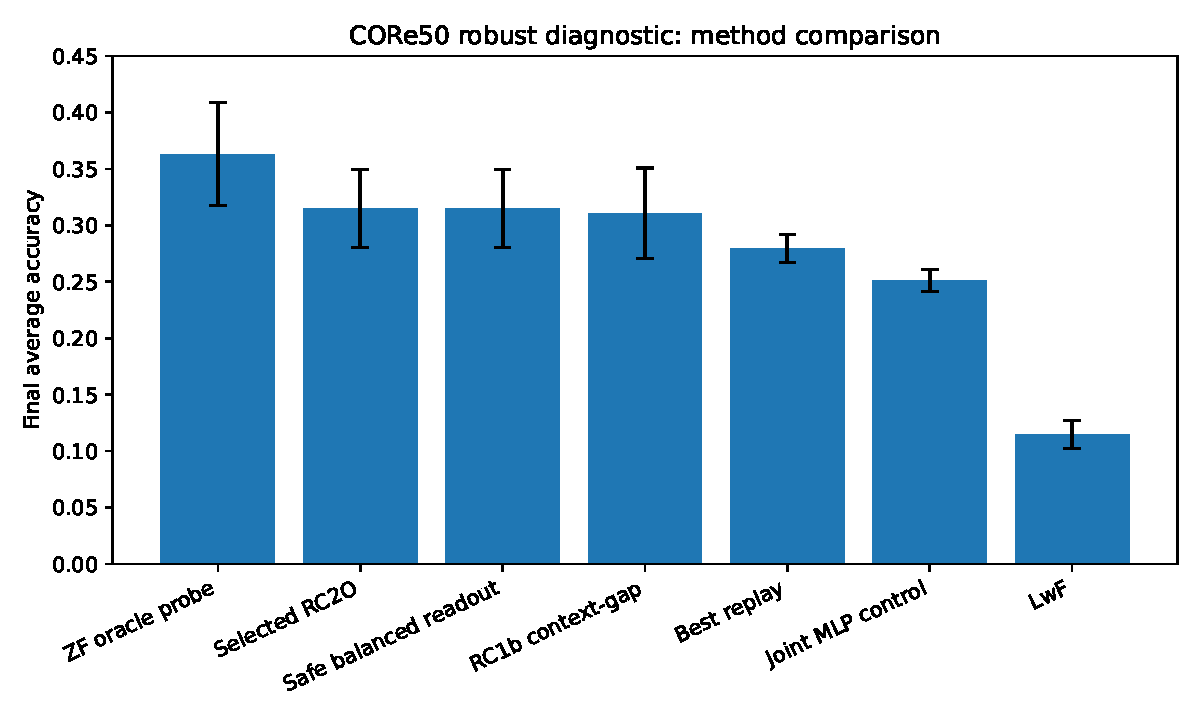
\includegraphics[width=\linewidth]{figures/core50_method_comparison.pdf}
\caption{Five-seed method comparison.}
\end{subfigure}\hfill
\begin{subfigure}{0.48\linewidth}
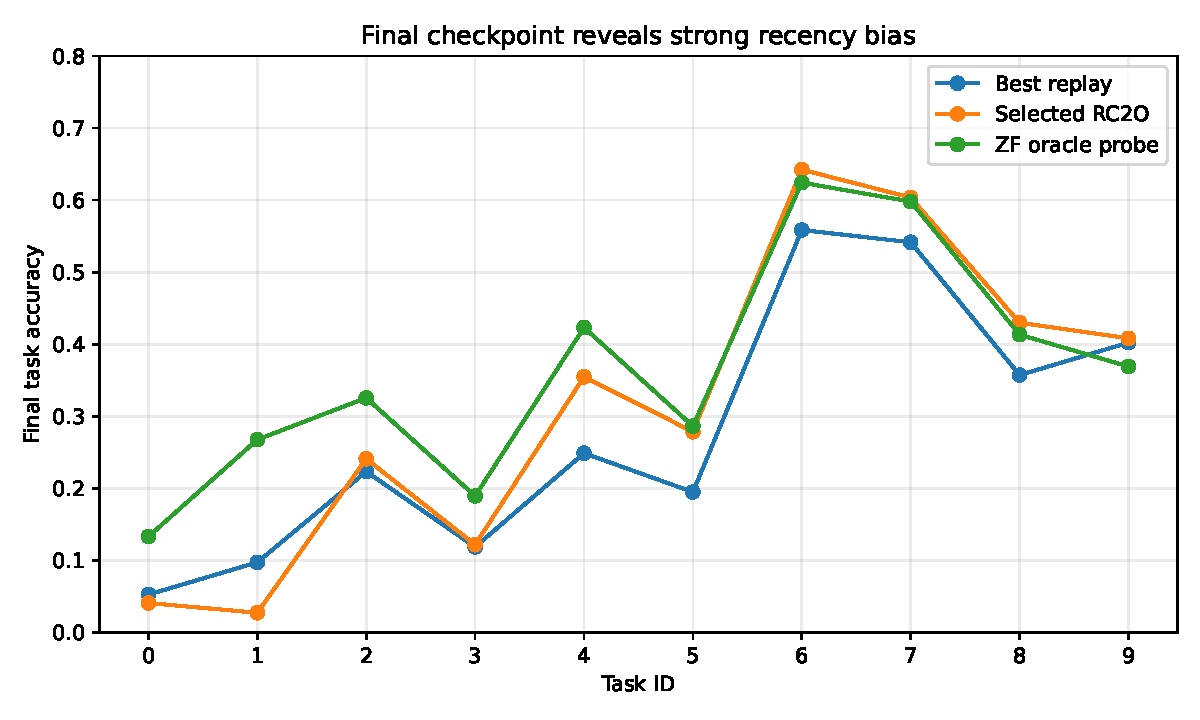
\includegraphics[width=\linewidth]{figures/core50_taskwise_recency.pdf}
\caption{Final taskwise recency profile.}
\end{subfigure}
\caption{\core{} robust diagnostic. Average accuracy improves, but earliest tasks nearly disappear.}
\end{figure}

The average conceals severe nonuniformity. Mean minimum-task accuracy is only $0.0146$, compared with $0.0527$ for replay. Early contexts are frequently assigned with near-zero entropy to the newest context. Yet the oracle-context probe reaches only $0.36305$, about $0.048$ above selected \rc{}, so context error is not the only bottleneck. Latent-function preservation, replay balance, readout geometry and feature capacity also limit performance.

The specialization audit also reveals a seed with almost complete one-host collapse. Therefore, the run supports external transfer and a modest reproducible paired gain, but not strong retention, standard \core{} benchmark comparability, or robust host specialization.

\section{CORe50 v2.3: failure-driven rescue ablation}
The v2.3 experiment does not repeat the unchanged five-seed run. It tests three variants on seed 0 and the route-collapse seed 4:
\begin{enumerate}[leftmargin=*]
\item the v2.2c reference;
\item context EMA retention with old-task replay;
\item a full rescue combining stronger representation, ten hosts, host balance, replay, proxy repair and dynamic readout.
\end{enumerate}

\begin{table}[H]
\centering
\caption{Mean v2.3 rescue results over seeds 0 and 4.}
\begin{tabular}{@{}lrrrrrr@{}}
\toprule
Variant & Avg. acc. & Min task & Oldest 2 & Context top-1 & Zero recall & Forgetting \\
\midrule
Reference v2.2c & 0.2734 & 0.0050 & 0.0274 & 0.5284 & 9.0 & 0.2223 \\
Context EMA retention & 0.2970 & 0.0010 & 0.0203 & 0.5724 & 10.5 & 0.2101 \\
Full rescue & \textbf{0.3171} & \textbf{0.0513} & \textbf{0.0560} & \textbf{0.7108} & \textbf{0.5} & \textbf{0.1499} \\
\bottomrule
\end{tabular}

\end{table}

\begin{figure}[H]
\centering
\begin{subfigure}{0.32\linewidth}
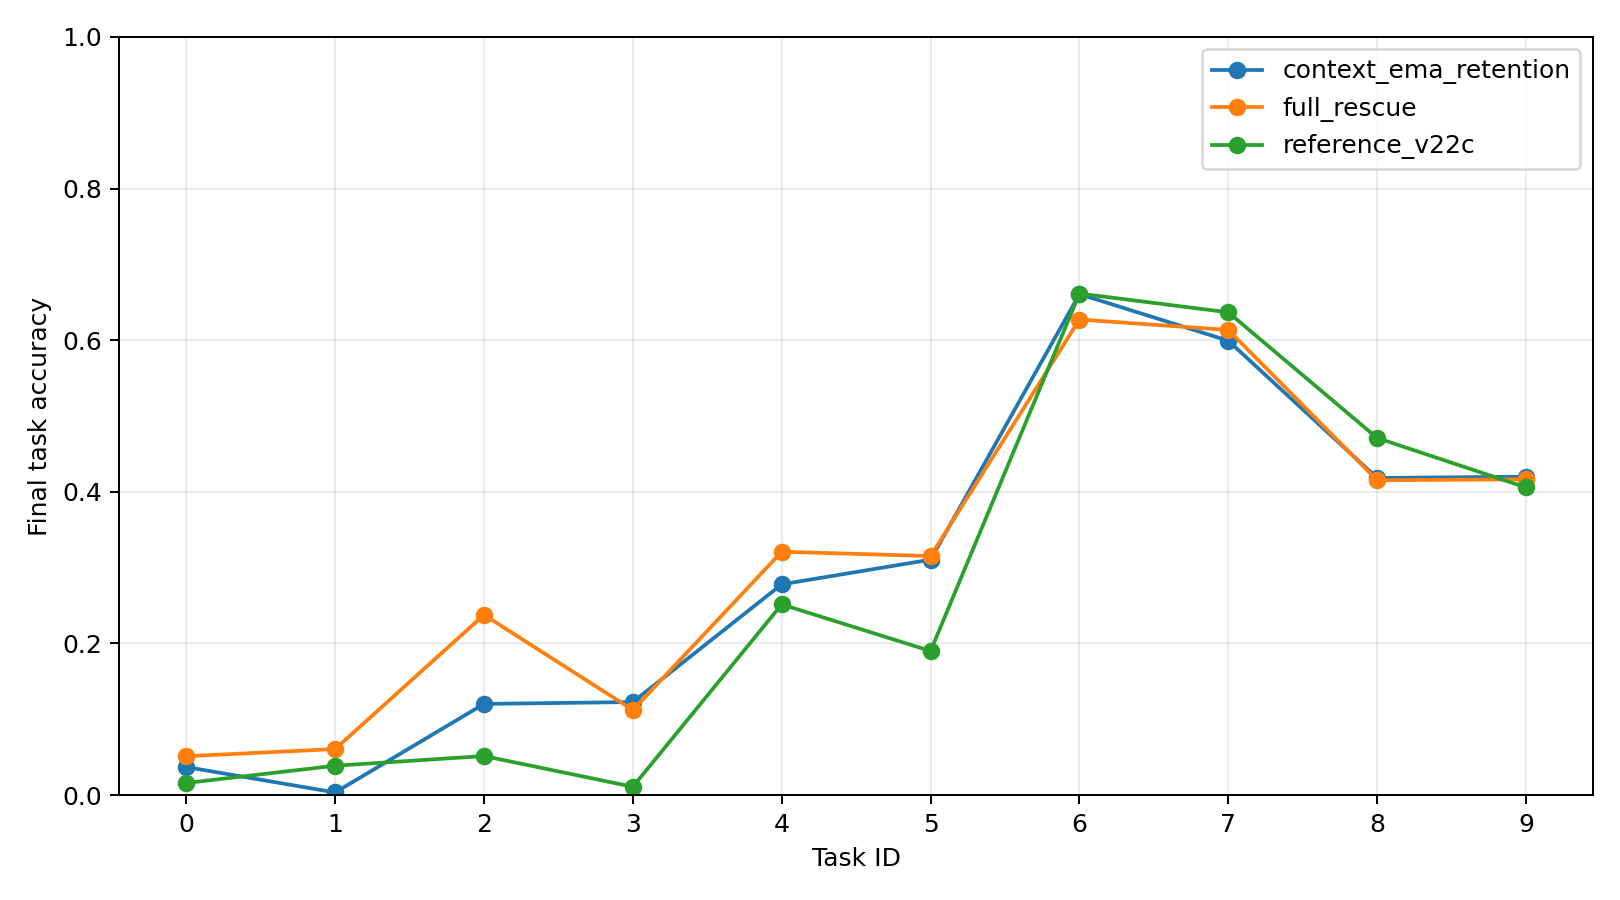
\includegraphics[width=\linewidth]{figures/final_task_accuracy_by_variant.png}
\caption{Task retention.}
\end{subfigure}\hfill
\begin{subfigure}{0.32\linewidth}
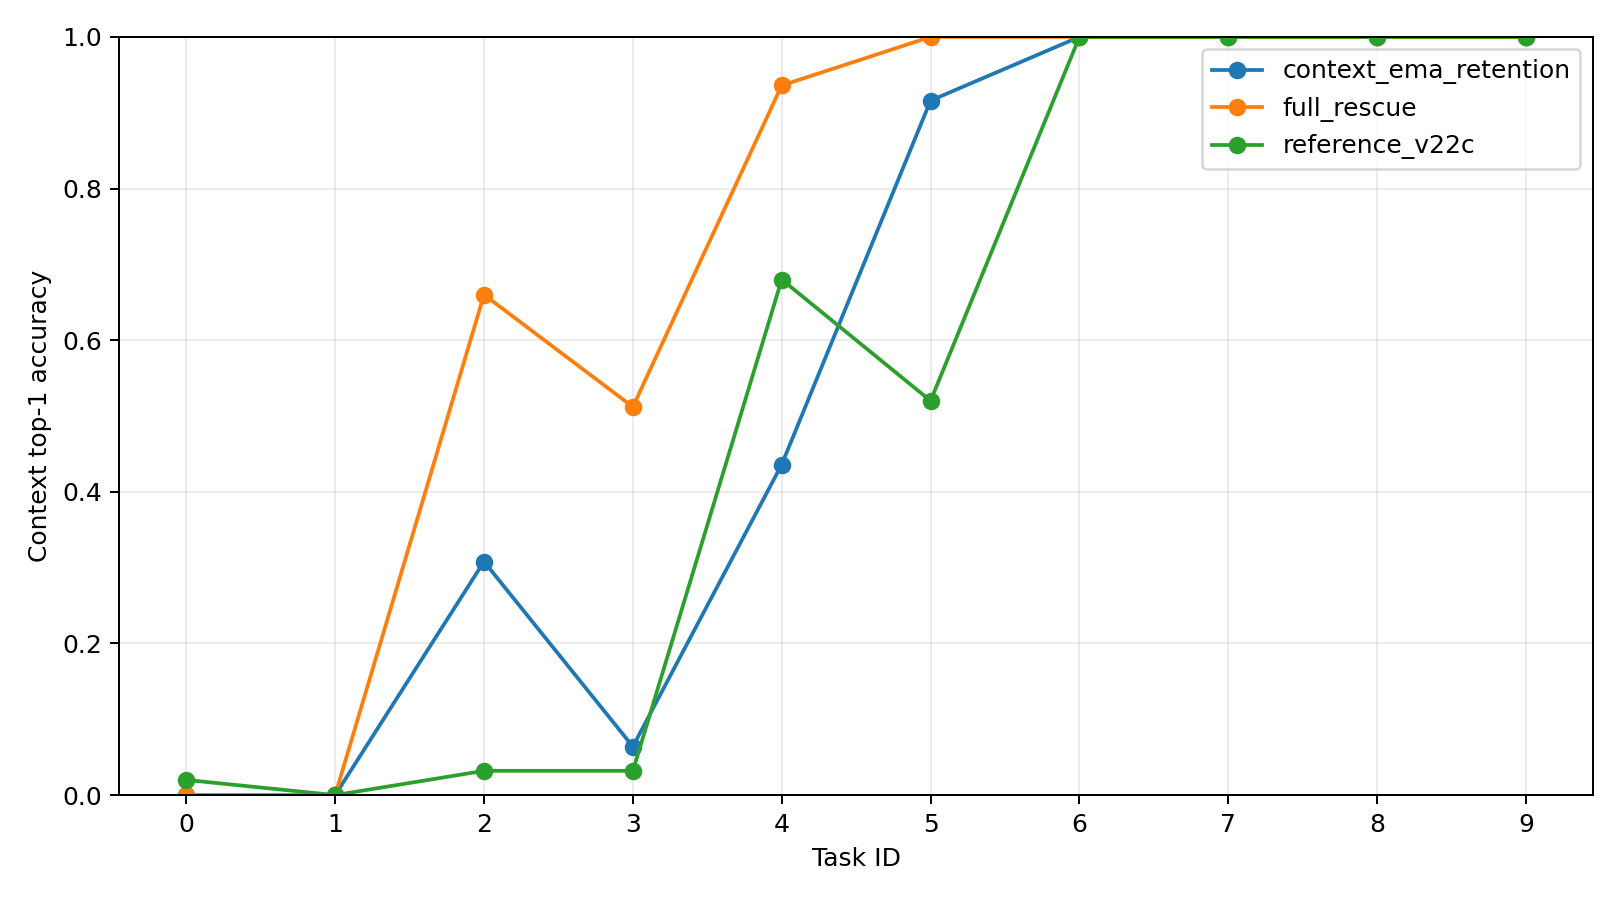
\includegraphics[width=\linewidth]{figures/context_retention_by_variant.png}
\caption{Context retention.}
\end{subfigure}\hfill
\begin{subfigure}{0.32\linewidth}
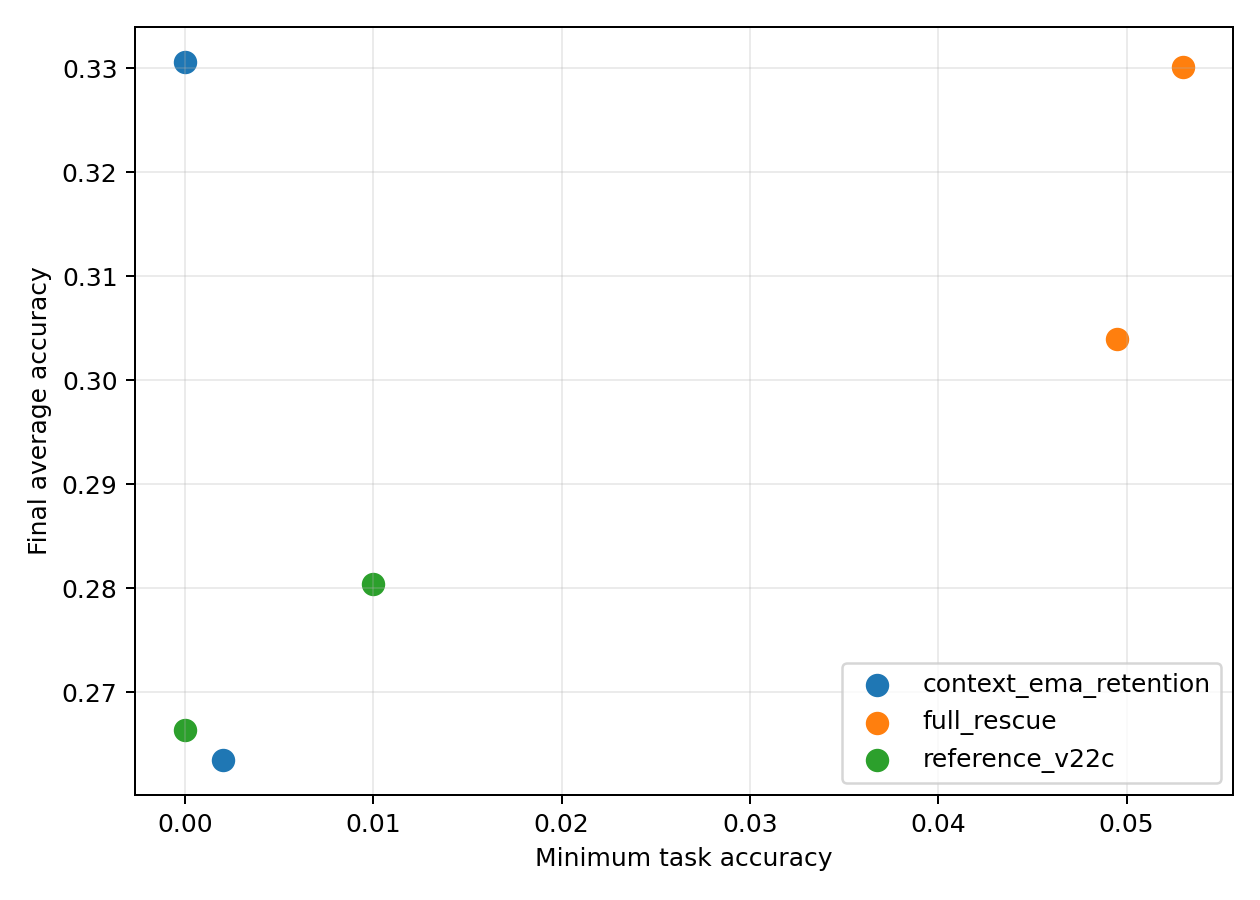
\includegraphics[width=\linewidth]{figures/retention_accuracy_tradeoff.png}
\caption{Trade-off.}
\end{subfigure}
\caption{CORe50 v2.3 rescue diagnostics.}
\end{figure}

The full rescue raises final average accuracy by $+0.0437$, minimum-task accuracy by $+0.04625$, reduces average forgetting by about $0.0724$, and reduces mean zero-recall classes by $8.5$. Effective hosts increase from approximately $2.04$ to $8.68$, while maximum route dominance falls from $0.956$ to $0.264$. This is a substantive partial success.

However, the isolated context EMA variant reduces oldest-task retention and increases zero-recall classes. More importantly, oldest-two context top-1 remains zero under the full rescue. The promotion gate therefore correctly returns \texttt{iterate\_before\_robust}.

\begin{table}[H]
\centering
\caption{Promotion-gate evidence.}
\begin{tabular}{@{}lrrrl@{}}
\toprule
Variant & Oldest-2 gain & Old-context gain & Zero-recall reduction & Decision \\
\midrule
Context EMA retention & -0.0071 & -0.0100 & -1.5 & Iterate \\
Full rescue & +0.0286 & -0.0100 & +8.5 & Iterate before robust \\
\bottomrule
\end{tabular}

\end{table}

\section{What the newest run teaches}
The v2.3 result isolates a mismatch between training and deployment. The retention loss directly trains a single-input context encoder, whereas the deployed posterior is dominated by a prototype-based branch. Consequently, the loss improves a component that contributes only weakly to the final decision, while the dominant prototype decision is not directly optimized by the retention objective.

This observation changes the next research question. The problem is no longer merely ``increase EMA strength'' or ``add more replay.'' It is:
\begin{quote}
How can the system preserve old context evidence while remaining plastic, train the posterior actually used at inference, and retain exact backward compatibility with prior results?
\end{quote}

The proposed answer is a dataset-agnostic stable-plastic context-memory module with three operating modes: \texttt{legacy}, \texttt{stable\_plastic}, and \texttt{adaptive}. The companion design note specifies the architecture, losses, regression gates and implementation contract. Importantly, the legacy path must reproduce earlier results without requiring users to recover historical notebooks.

\section{Claim boundary}
\begin{table}[H]
\centering
\caption{Supported and unsupported external claims.}
\begin{tabularx}{\linewidth}{@{}p{0.28\linewidth} p{0.30\linewidth} X@{}}
\toprule
Evidence & Supported statement & Unsupported extrapolation \\
\midrule
SplitCIFAR10 robust & RC2O substantially outperforms validation-selected replay with low forgetting and no class collapse over frozen A1 features. & End-to-end raw-pixel continual representation learning or CIFAR state of the art. \\
SplitCIFAR100 robust diagnostic & RC2O has a large paired advantage over replay. & Full qualification, because representation and joint-control floors remain weak. \\
CORe50 robust diagnostic & The external pipeline transfers and yields a modest positive paired gain in every seed. & Strong retention, standard CORe50 NC/NIC comparability, or proven host specialization. \\
CORe50 v2.3 rescue & Combined representation, replay, readout and host changes reduce zero-recall classes, forgetting and host collapse. & Attribution to context EMA or successful oldest-context retention. \\
\bottomrule
\end{tabularx}

\end{table}

No positive backward transfer claim is made. The \core{} stream is custom and not equivalent to a standard NC or NIC benchmark. The current external experiments use frozen visual representations, so they do not validate sequential acquisition of unseen visual features. Several controls named ``joint upper bound'' in raw notebooks are reported here as \emph{joint MLP controls}; because \rc{} can exceed them, they are not theoretical upper bounds.

\section{Program roadmap}
The next sequence is deliberately conservative:
\begin{enumerate}[leftmargin=*]
\item implement the stable-plastic context-memory module behind an exact legacy mode;
\item test mechanism variants on \core{} seeds 0 and 4;
\item run one-seed regression smokes on MNIST, FashionMNIST, RotatedMNIST and PermutedMNIST;
\item protect the qualified \scx{} result with strict non-regression gates;
\item revisit \scxx{} as a diagnostic with stronger representation and readout controls;
\item run a new five-seed \core{} robust experiment only after context-specific gates pass.
\end{enumerate}

\section{Reproducibility package}
The GitHub package contains this source and compiled PDF, selected figures, machine-readable evidence for \scx{}, \scxx{}, \core{} and v2.3, the key executed notebooks, claim-boundary notes, checksums, and build instructions. Large raw score dumps and full 100+ MB run archives are intentionally excluded from repository hygiene; the original run packages remain separate evidence artifacts.

\section{Conclusion}
The current evidence does not support the statement that \mmals{} has solved continual learning. It supports a more precise progression. Functional-memory diagnostics on the MNIST family established that route topology is not sufficient. \scx{} provides robust external-bridge evidence over frozen visual features. \scxx{} and \core{} show that the same architecture can transfer, but also expose representation, readout, context-retention and specialization limits. The v2.3 rescue substantially reduces class and host collapse yet fails its oldest-context target. That failure is scientifically productive: it identifies a localized, testable redesign while preserving the rest of the \mmals{} backbone and its audit discipline.

\begin{thebibliography}{12}
\bibitem{parisi2019} G. I. Parisi, R. Kemker, J. L. Part, C. Kanan, and S. Wermter. Continual lifelong learning with neural networks: A review. \emph{Neural Networks}, 113:54--71, 2019.
\bibitem{kirkpatrick2017} J. Kirkpatrick et al. Overcoming catastrophic forgetting in neural networks. \emph{PNAS}, 114(13):3521--3526, 2017.
\bibitem{li2016} Z. Li and D. Hoiem. Learning without forgetting. \emph{ECCV}, 2016.
\bibitem{rusu2016} A. A. Rusu et al. Progressive neural networks. \emph{arXiv:1606.04671}, 2016.
\bibitem{shazeer2017} N. Shazeer et al. Outrageously large neural networks: The sparsely-gated mixture-of-experts layer. \emph{ICLR}, 2017.
\bibitem{rebuffi2017} S.-A. Rebuffi, A. Kolesnikov, G. Sperl, and C. H. Lampert. iCaRL: Incremental classifier and representation learning. \emph{CVPR}, 2017.
\bibitem{lomonaco2017} V. Lomonaco and D. Maltoni. CORe50: A new dataset and benchmark for continuous object recognition. \emph{CoRL}, 2017.
\bibitem{mmals09} G. Harbonnier. MMALS Prototype v0.9: Route-function disentanglement. Internal reproducibility artifact, 2026.
\bibitem{mmals12} G. Harbonnier. MMALS Prototype v0.12: Hopfield co-evolution evidence. Internal reproducibility artifact, 2026.
\bibitem{mmalssc10} G. Harbonnier. MMALS RC2O-v2.2c SplitCIFAR10 robust package. Internal reproducibility artifact, 2026.
\bibitem{mmalssc100} G. Harbonnier. MMALS RC2O-v2.2c SplitCIFAR100 robust diagnostic addendum. Internal reproducibility artifact, 2026.
\bibitem{mmalscore50} G. Harbonnier. MMALS RC2O-v2.2c CORe50 robust diagnostic and v2.3 rescue packages. Internal reproducibility artifacts, 2026.
\end{thebibliography}
\end{document}
